Here \ref{dist1plot} \ref{dist6plot}
\begin{figure}
    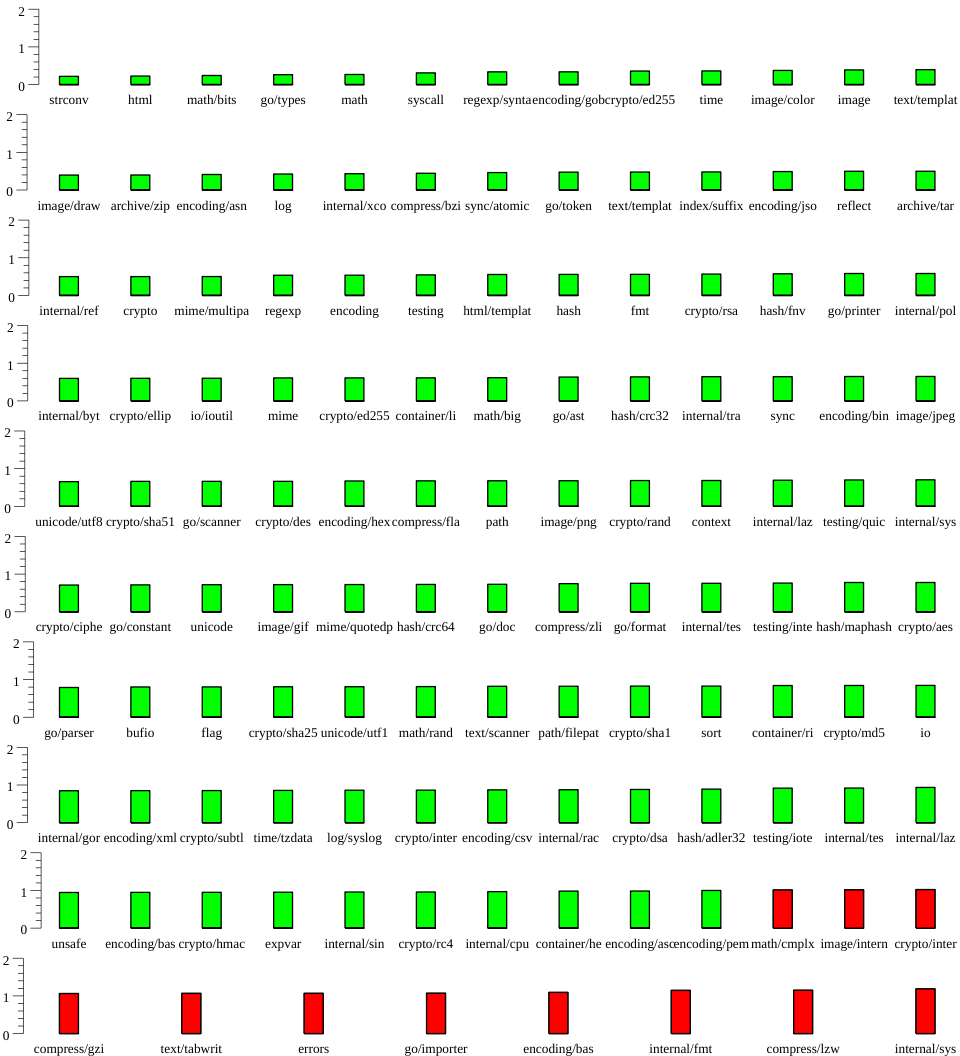
\includegraphics[width=\textwidth]{example1.png}
    \label{dist1plot}
    \centering
    \caption{Each Go module was indexed and then randomly queried.
    Speed up over linear search for a search distance of $1$ is plotted for each Go module.
    Green idicates search was fater, red otherwise.
    Names are the first twelve characters of module name.
    The rest are elided for readability.}
\end{figure}
\begin{figure}
    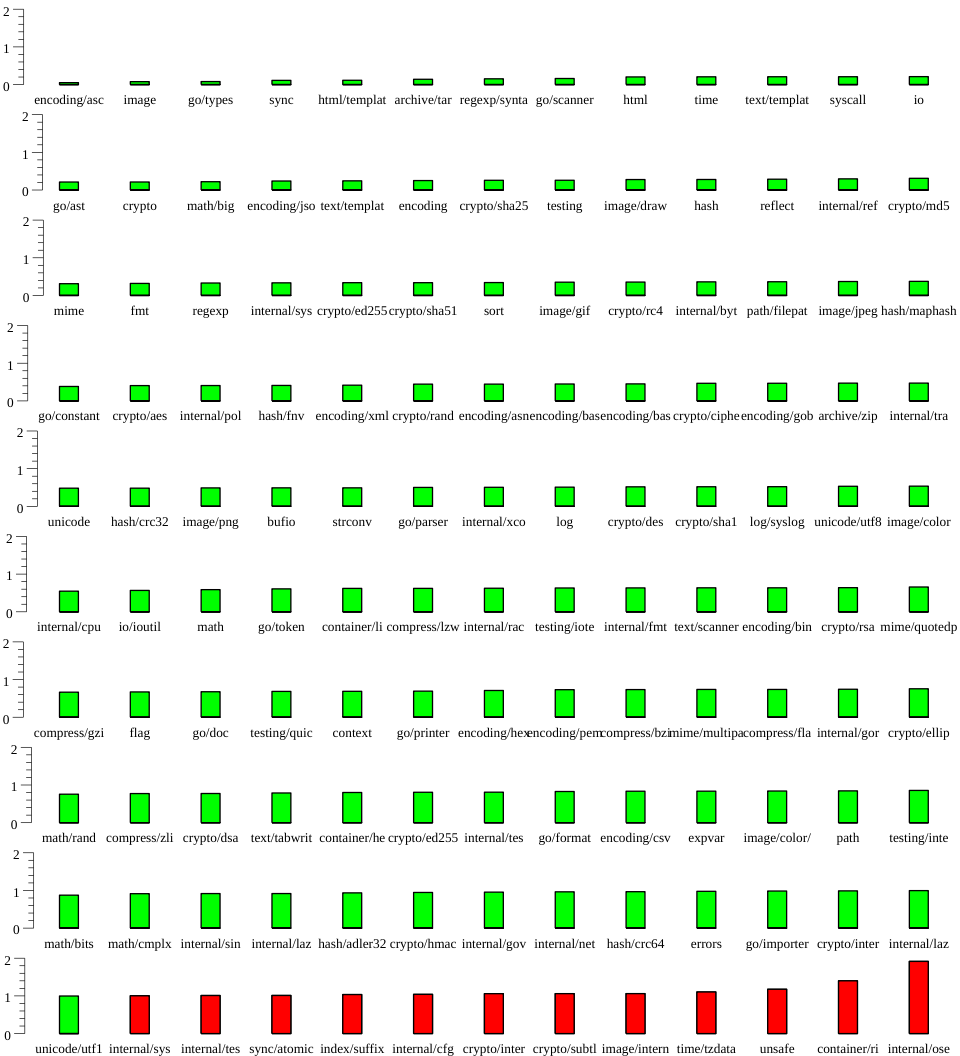
\includegraphics[width=\textwidth]{example6.png}
    \label{dist6plot}
    \centering
    \caption{Each Go module was indexed and then randomly queried.
    Speed up over linear search for a search distance of $6$ is plotted for each Go module.
    Green idicates search was fater, red otherwise.
    Names are the first twelve characters of module name.
    The rest are elided for readability.}
\end{figure}